% LREC Document Attrition paper, based on ACL2005 example TeX


\documentclass[10pt, a4paper]{article}
% =============================================================================
% Package inclusions
\usepackage{lrec2014}
\usepackage{times}
\usepackage{graphicx}

\usepackage{xcolor}

\usepackage{fancyvrb}

\usepackage[hidelinks]{hyperref}

% =============================================================================
% Custom commands
%\setlength\titlebox{6.5cm}    % Expanding the titlebox

\newcommand{\superscript}[1]{\ensuremath{^{\textrm{#1}}}}
\newcommand{\subscript}[1]{\ensuremath{_{\textrm{#1}}}}
\newcommand{\mon}[1]{{\tt #1}}

% Draft colour
% use \dr{stuff you want redrafting} to highlight something.
\newcommand{\dr}[1]{{\color{blue} #1}}%

% =============================================================================
% Package config
\graphicspath{{./images/}}
\DeclareGraphicsExtensions{.pdf,.png,.jpg}


% =============================================================================
% Title and header content; metadata
% \title{Experiences Scaling an Existing NLP Toolkit: Hansard and USAS}
\title{Experiences with Parallelisation of an Existing NLP Pipeline: Tagging Hansard}

% Confirmation Number:	 687
% Submission Passcode:	 687X-D2C3A3A6J3


\name{Stephen Wattam\superscript{\small{1}}, Paul Rayson\superscript{\small{1}}, Marc Alexander\superscript{\small{2}} \& Jean Anderson\superscript{\small{2}}}


\address{School of Computing and Communications\superscript{\small{1}} \\
Lancaster University \\
{\tt \{s.wattam, p.rayson\}@lancaster.ac.uk}
\and
	English Language\superscript{\small{2}} \\
University of Glasgow \\
	{\tt \{marc.alexander, jean.anderson\}@glasgow.ac.uk}}


% =============================================================================
\abstract{    This poster describes experiences processing the two-billion-word Hansard corpus using a fairly standard NLP pipeline on a high performance cluster.  Herein we report how we were able to parallelise and apply a ``traditional'' single-threaded batch-oriented application to a platform that differs greatly from that for which it was originally designed. We start by discussing the tagging toolchain, its specific requirements and properties, and its performance characteristics.  This is contrasted with a description of the cluster on which it was to run, and specific limitations are discussed such as the overhead of using SAN-based storage. We then go on to discuss the nature of the Hansard corpus, and describe which properties of this corpus in particular prove challenging for use on the system architecture we used. The solution for tagging the corpus is then described, along with performance comparisons against a na\"{i}ve run on commodity hardware.  We discuss the gains and benefits of using high-performance machinery rather than relatively cheap commodity hardware. Our poster provides a valuable scenario for large scale NLP pipelines and lessons learnt from the experience.


% My collided edit:
%
% This poster describes experiences gained in adapting the USAS semantic tagger for use on the Lancaster University high-end computing (HEC) cluster.  We describe the process of tagging the Hansard corpus, comprising 2.2 billion words, by parallelising the existing toolchain: a ``traditional'' single-threaded, batch-oriented system originally designed for execution on low-resource desktop machines.\\
%     We start by discussing the tagging toolchain, its specific requirements and properties, and its performance characteristics.  This is contrasted with a description of the cluster on which it was to run, and specific limitations are discussed, such as the overheads involved in scheduling jobs and accessing SAN-based storage arrays.\\
%     The structure of the Hansard corpus is then described, and it is assessed to identify which aspects prove challenging for use on the cluster.  We describe the solution found, and compare its performance to that of a conventional desktop system in order to evaluate the efficacy of the parallelisation effort.
%     We conclude that many data sets and toolchains may benefit only a little from parallelisation due to the development overhead required, but that this particular data set benefitted greatly from the increased performance high-performance computing hardware affords.
% 



 \vspace{11pt} \Keywords{High-performance Computing, Parallelisation, Tagging}}





% =============================================================================
% Document body
\begin{document}
\maketitleabstract%

% -------------------------------------------------------------------
\section{Introduction}
Requirements for NLP processing systems now typically include the need for extremely large scale processing of data derived either from vast online sources or increasing quantities of digitised archive material. 
Whether the scenario is to answer a particular set of research questions or for commercial text analytics, sources such as Twitter provide significantly more data than can be processed and ingested in anything like reasonable time. Parallel computation is typically used to address this bottleneck. 
This poster presents the lessons learnt from our work which emerged from two serendipitous events. First, the need to support digital humanists in their analysis of the full Hansard data set and second a need for a real case study for Lancaster University's High Performance Cluster using textual rather than numerical data. Large infrastructure activities such as CLARIN~\cite{varadi2008clarin} and DARIAH~\cite{constantopoulos2008preparing} are providing distributed archives for language resources but NLP research teams still face local requirements during experimentation to process and reprocess very large resources through complex pipelines. Some toolkits, e.g. GATE can now run in the cloud~\cite{tablan2013gatecloud} to suport such activities. However, many universities have existing high performance clusters that may be under exploited by language researchers. 

% \dr{Todo: signposting}


% -------------------------------------------------------------------
\section{Toolchain}
The toolchain being used to tag the corpora was a combination of tools comprising the tag wizard of the Wmatrix system\footnote{\url{http://ucrel.lancs.ac.uk/wmatrix/}}.  
This consists of a number of tagging and analysis tools, each communicating using intermediate files and managed using a series of shell scripts.  
The tag wizard shares a lot of commonalities with standard NLP processing pipelines as it consists of two annotation systems (CLAWS and USAS) plus a frequency profiling and keyness comparison step.



% -------------------------------------------------------------------
\section{High-Performance System}
The system used for processing was the Lancaster university High-End Computing cluster (HEC).  This consists of a number of compute nodes running Scientific Linux, connected using the Sun Grid Engine.  In total the system comprises over 2200 CPU cores, 11TB of memory, 32TB of high performance (working) file storage, and a further 1PB of medium performance storage.


\begin{figure}[h]
\centering
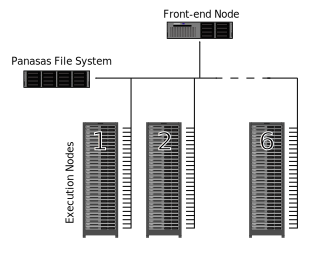
\includegraphics[width=0.5\textwidth]{arch.png}
\caption{HEC architecture}
\label{fig:arch}
\end{figure}

As shown in figure~\ref{fig:arch}, the system is reliant on network-attached shared storage in the form of a Panasas Activescale Series 8 storage cluster.  Intermediate storage is provided by a number of other storage nodes \todo{Do these provide the working shared storage/scratch, or are they only for use with GridPP?}.

There are 262 compute nodes in total, each with two four- or six-core CPUs\todo{Xeons?} each.  Most of these compute nodes have 24GB of RAM available locally (those that do not have 96GB).

Jobs are deployed on the HEC using the Sun Grid Engine scheduling framework, and works in a batch processing manner.  Jobs contend with one another for access to compute nodes.  This scheduler can be used to queue up job arrays in large batches, which will then be distributed to each compute node individually as they become free.  This was the primary mechanism used to distribute jobs across nodes.




% -------------------------------------------------------------------
\section{Hansard Corpus}
\dr{
About the corpus origins, aims, format.
}

\begin{itemize}
    \item Size
        \begin{itemize}
            \item 7545103 XML files in 48,482 directories comprising 2,271,985,142 words and 32.7952GiB of data [inc markup].
            \item Word sizes: 40, 83, 147, 308, 1400 at 5\%, 25\%, 50\%, 75\% and 95\%.
            % > quantile(words$words, c(.05, .25, .50, .75, .95))
            %   5%  25%  50%  75%  95% 
            %   40   83  147  308 1400
            \item Average filesize is 2.4KB
            \item Totals and breakdowns
        \end{itemize}
    \item Format
        \begin{itemize}
            \item Individual files
            \item folder structure and organisation (pertinent to later organisation/batching)
        \end{itemize}
\end{itemize}

\subsection{Format}
The corpus is split into 7,545,103 XML files, each representing a speech made in either house of the UK Parliament.  These files are organised into a hierarchical directory structure by house and date.  A sample of this structure is shown in Figure~\ref{fig:structure}.

\begin{figure}[h]
    \centering
    {
        \small
        \begin{Verbatim}[frame=single]
            Hansard
            +-- Commons
            |   +-- commons 1803-1820
            |   |   \-- commons
            |   |       +-- 1803
            |   |       |   +-- dec
            |   |       |   |   +-- 01
            |   |       |   |   +-- 02
            |   |       |   |   +-- 03
            |   |       |   |   +-- 05
            |   |       |   |   +-- ...
        \end{Verbatim} 
    }
    \caption{Sample directory layout}
    \label{fig:structure}
\end{figure}


\begin{figure}[h]
    \centering
    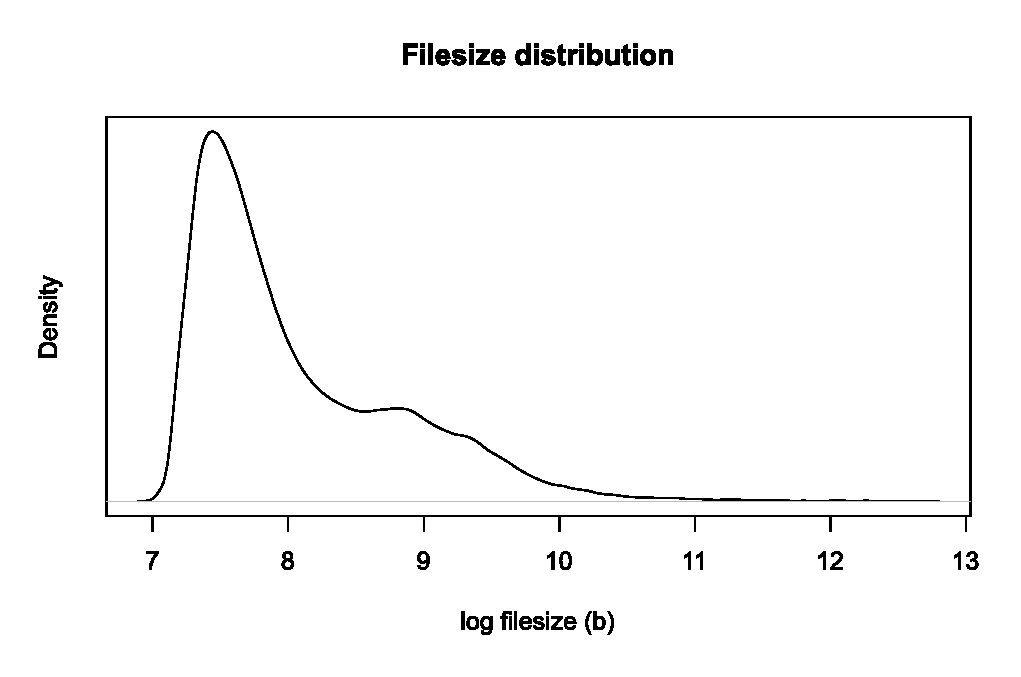
\includegraphics[width=0.5\textwidth]{filesize.eps}


    \begin{tabular}{ | r | c | c | c | c | c | }
        \hline
        Percentile & 5 & 25 & 50 & 75 & 95 \\ \hline
        Words & 40 & 83 & 147 & 308 & 1400 \\ \hline
    \end{tabular}

    \caption{Distribution of log filesizes for all corpus data, and word counts (without markup) for each file.}
    \label{fig:filesizes}
\end{figure}


\dr{The XML format used contains annotations for X, Y and Z, and follows various conventions...  }

The XML files themselves follow x format\todo{unsure of this, SW}. File sizes are distributed in a Zipfian manner, as shown in Figure~\ref{fig:filesizes}. The median size is just 2.4KB, and the 95th percentile is 1.4MB.


% \begin{verbatim}
% > quantile(sizes$filesize, c(.05, .25, .50, .75, .95))
%    5%   25%   50%   75%   95% 
%  1411  1781  2443  5031 14013
% \end{verbatim}


\subsection{Tagging}
\begin{itemize}
    \item What needed tagging
    \item Which frequencies had to be built (per file/day/totals)
    \item What work this contributed to
\end{itemize}



% -------------------------------------------------------------------
\section{Method}
\subsection{Limitations \& Solutions}
\begin{itemize}
    \item Small files (filesystem overhead)
        \begin{itemize}
            \item Input files [tarred, stored in RO storage]
            \item Temp files and toolchain comms [on nodes]
            \item Output file storage [tarred, stored on shared disk after tarring]
        \end{itemize}
    \item Small jobs (job overhead)
        \begin{itemize}
            \item Batching using ID numbers
            \item Scheduling to distribute load (many jobs, composite job thing)
        \end{itemize}
    \item Co-ordination of parallel tasks
        \begin{itemize}
            \item Use of a pre-built index
            \item batches of fixed size, job ID computes offset
        \end{itemize}
\end{itemize}



\subsection{Final Method}
\begin{itemize}
    \item Corpus pre-tarred into daily runs so as to avoid filesize issues and problems with multiple-directory structure
    \item Corpus stored in read-only space due to size
    \item Everything compiled in ~/.local directory on server, batch scripts set up for toolchain in new shell
    \item Produce directory listing of input file groups
    \item Batch file
        \begin{itemize}
            \item Computes batch size from batch ID
            \item Duplicates directory tree in the working compute node
            \item extracts everything
            \item Runs pipeline over each file
            \item Archives results 
            \item Archives all of those results to produce a large file for storage on panasas shelf
            \item Copies back
            \item Deletes compute node
            \item Stores stdout/stderr in common location with batch ID
        \end{itemize}
    \item Output structure taken off HEC
    \item Validation script tests:
        \begin{itemize}
            \item output files exist
            \item The right number of files is in the output/input tars
            \item File sizes are nonzero
        \end{itemize}
\end{itemize}






% -------------------------------------------------------------------
\section{Performance}
% \begin{itemize}
%     \item When moving processing to a high performance cluster there are two main gains:
%         \begin{itemize}
%             \item Parallelism, which greatly benefits this problem as it is 'embarrassingly parallel'
%             \item Serial speed of each compute node (clusters are usually well specified w.r.t. RAM and CPU provisions)
%         \end{itemize}
% \end{itemize}
% 
% 
% 
% 
% 
% \subsection{HEC}

\begin{figure}[h]
    \centering
    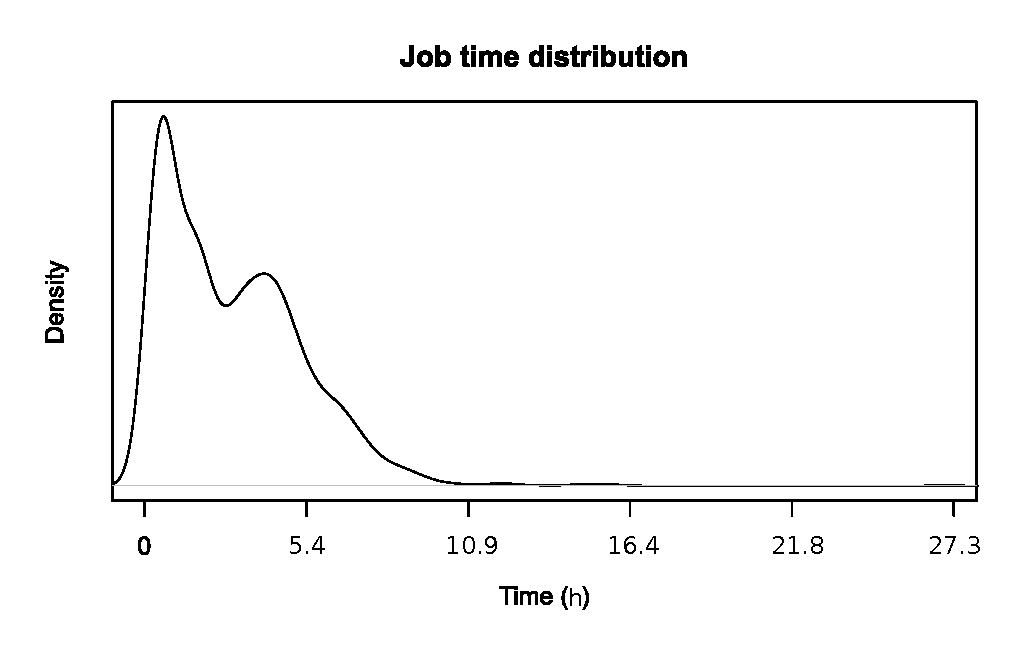
\includegraphics[width=0.5\textwidth]{jobtime.eps}

    \begin{tabular}{ | r | c | c | c | c | c | }
        \hline
        Percentile & 5 & 25 & 50 & 75 & 95 \\ \hline
        Duration & 20m & 53m & 2.5h & 4.5h & 7.3h \\ \hline
    \end{tabular}

    \caption{Distribution of job execution times on the HEC}
    \label{fig:jobtimes}
\end{figure}


% 
% {\small
% \begin{verbatim}
% Total time (s): 24428748    ( / 60 / 60 / 24 = 282 days on the HPC )
% Mean (s): 10955             ( / 60 / 60 = 3.04 hours )
% Min (s): 223                ( / 60 = 3.7 minutes )
% Max (s): 98872              ( / 60 / 60 = 27 hours )
% 
% 
% > quantile(x$time, c(.05, .25, .50, .75, .95))
%        5%       25%       50%       75%       95% 
%  1248.897  3174.155  9321.105 16462.717 26126.913 
%  20 mins   53 mins   2.5 hrs  4.5 hrs   7.25hrs
% \end{verbatim}
% }
% 




All jobs were complete in 3 days, meaning that the system tagged at a rate of 31.5 million words 
%31,555,349 words 
per hour.  Because of the heterogeniety in task length, this rate was not constant, decaying towards the end (the final 231) as the queued tasks ran out and were not replaced.  Had we used larger batches, this effect would have proven more severe as the variance in job length was liable to increase.  Were the corpus particularly large (in the range of hundreds of billions of words), it would be prudent to model and control for this effect ahead of time.
Jobs used a maximum of between 80 and 120MB of memory---our greatest underutilised resource.
% It should be possible to improve the tagging rate by further parallelising within each compute node.  This would theoretically shorten the time spent tagging by a factor of at least 8 to just 9 hours.

% Note that, in order to be evenly divisible by 20, the task list was padded.  This makes the minimum task execution time smaller than it would otherwise be.



\subsection{Commodity Hardware}
In many cases, the alternative to deployment on a HEC cluster will be use of one or many commodity desktop machines.  In order to compare the performance of the toolchain, a random sample of 50 jobs was run through the toolchain using the scheduling scripts described above.

The hardware used was a desktop machine with a single Intel i5 processor, 15GB of memory, and two 7200rpm mechanical hard disks in a RAID-0 configuration.  The system was running Arch Linux\footnote{\url{http://archlinux.org}}, and, as the system is the first author's office machine, work continued on other projects during the benchmarks.  We believe this constitutes a system equivalent to many found across offices today.

\begin{figure}[h]
    \centering
    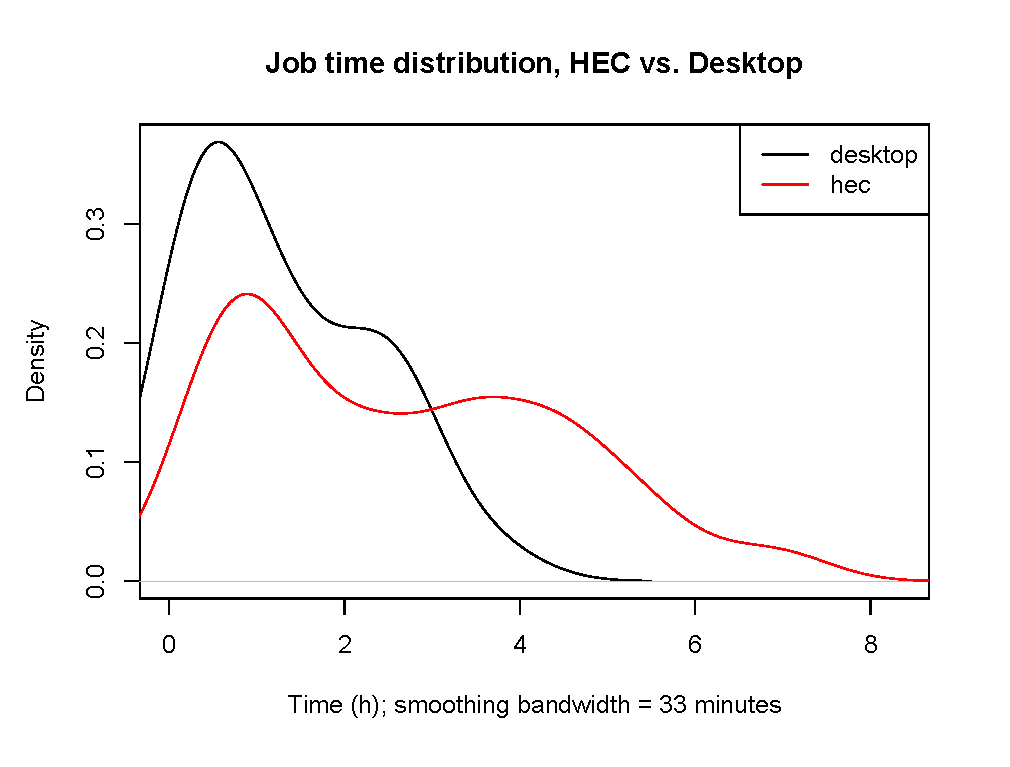
\includegraphics[width=0.5\textwidth]{timecomp.eps}
    % postscript("timecomp.eps", height=5, width=6.5)
    % plot(density(times$tdesk/3600, bw=2000/3600), xlim=c(0, 30000/3600), main="Job time distribution, HEC vs. Desktop", xlab="Time (h); smoothing bandwidth = 33 minutes")
    % lines(density(times$thec/3600, bw=2000/3600), col=2)
    % legend("topright", c("desktop", "hec"), lty=1, col=c(1,2))
    % dev.off();

    % -------------
    % > quantile(times$thec, c(.05, .25, .50, .75, .95))
    %        5%       25%       50%       75%       95% 
    %  1322.534  3404.690  8524.075 14848.393 20306.699 
    % > quantile(times$tdesk, c(.05, .25, .50, .75, .95))
    %         5%        25%        50%        75%        95% 
    %   552.9762  1332.1664  3804.2810  8380.7053 10042.5802 

    \begin{tabular}{ | r | c | c | c | c | c | }
        \hline
        Percentile & 5 & 25 & 50 & 75 & 95 \\ \hline
        HEC        & 22m & 57m & 2.4h & 4.1h & 5.6h \\ \hline
        Desktop    & 9m & 22m & 1h & 2.3h & 2.8h \\ \hline
    \end{tabular}

    \caption{HEC and Desktop job execution times for a sample of 50 jobs}
    \label{fig:timecomp}
\end{figure}


As can be seen in Figure~\ref{fig:timecomp}, the desktop system runs individual jobs significantly faster.  Fitting a linear model indicates that the desktop is able to run jobs approximately 2.1 times faster than a single HEC core.  The same model indicates a 100 second job startup overhead on the HEC (including copying of files).
Had we continued to tag the corpus in this manner, it would have taken 98 days on the desktop system, and thus required at least 33 equivalent machines to achieve the HEC's performance.  It seems unlikely that manually splitting the data across that many systems would save time compared to the development overheads incurred for the HEC tagger.




% -------------------------------------------------------------------
\section{Discussion and conclusion}
\begin{itemize}
    \item Compare against the price of manually parallelising on a "few" commodity systems--
        \begin{itemize}
            \item Dev time
            \item Execution time
            \item Relative speed up
            \item Relative difficulty avoiding job overheads, etc.
        \end{itemize}
\end{itemize}

Though parallelisation undoubtedly saved countless hours, the design of the toolchain mandated significant manual intervention, and use of HEC machinery arguably did little to favour existing constraints.

Two weeks was spent developing and testing the HEC deployment of the toolchain.  Of this, a significant portion was spent adapting the toolchain to run on the scheduler without restriction from the shared filesystem.

The problem is embarrassingly parallel, but the HEC incurs severe overheads for some operations that are fast on commodity systems.  This effect is particularly noticable as the toolchain was designed with such systems in mind.  One possible alternative to use of such specialised hardware would be manually parallelising the toolchain over a number of desktop systems.  This has a number of advantages in terms of development time, and greatly simplifies the deployment in terms of software requirements (especially as a whole system can then be booted from cloned external disks or the network).  In situations where the toolchain to be run is not inherently parallel, and the problem is, this could prove a relative cheap, fast, and easy option.






% =============================================================================
\bibliographystyle{lrec2014}
\bibliography{hansard-lr14}

% =============================================================================
\end{document}

